\section{Audit results}\label{app:audit-results}
\subsection{Policy cost}
Audited teaching lowers initial-student cost by 7.74\% in mechanics
and 18.64\% in reaction, with five wins per task, but remains 0.42\%
and 2.60\% above the teacher (Table~\ref{tab:costs}). Student-minus-teacher
intervals are $[-0.012495,0.036137]$ and $[-0.021056,0.058030]$;
one mechanical and three reaction students beat their teachers.
\begin{table}[htbp]\centering\small\setlength{\tabcolsep}{4pt}
\begin{tabular}{@{}lrrrr@{}}\toprule
Task & Method & Cost & Updates & Audits\\\midrule
Mechanical & Teacher & 2.814376 & -- & --\\
Mechanical & Initial student & 3.063236 & -- & --\\
Mechanical & Cloning & 2.826377 & 28938 & 0.0\\
Mechanical & Cached H & 2.864541 & 29770 & 0.0\\
Mechanical & Selected fixed & 2.825197 & 29674 & 0.0\\
Mechanical & Adaptive & 2.829827 & 29766 & 0.0\\
Mechanical & Audit-guided & 2.826198 & 4019 & 31.4\\
Reaction & Teacher & 0.711506 & -- & --\\
Reaction & Initial student & 0.897189 & -- & --\\
Reaction & Cloning & 0.745016 & 21357 & 0.0\\
Reaction & Cached H & 0.822687 & 21507 & 0.0\\
Reaction & Selected fixed & 0.835997 & 21731 & 0.0\\
Reaction & Adaptive & 0.731010 & 21510 & 0.0\\
Reaction & Audit-guided & 0.729993 & 3232 & 25.2\\
\bottomrule\end{tabular}
\caption{Mean costs and computation under the common 30-second teaching
allocation, using five paired replications per task. Teacher and initial
student policies are pretrained inputs; their construction costs are separate.
All continuation audits and common preparation are charged.}
\label{tab:costs}
\end{table}

\begin{figure}[htbp]\centering
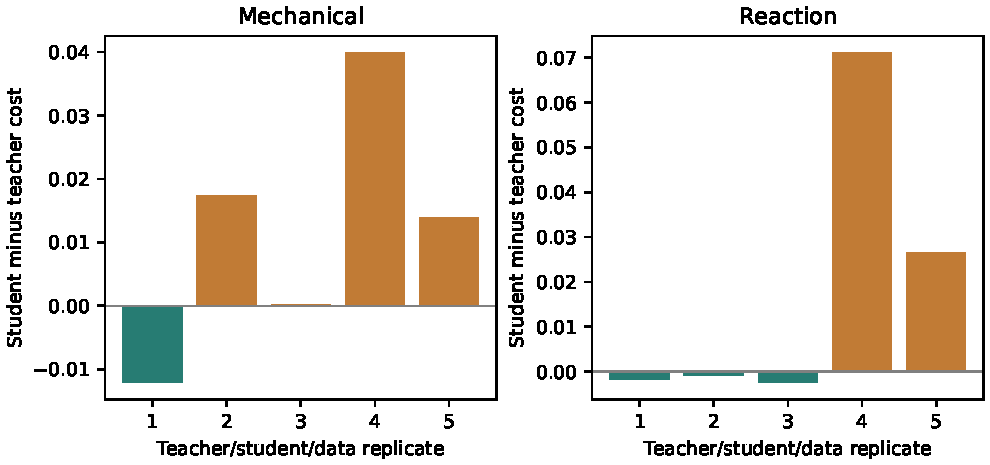
\includegraphics[width=\linewidth]{figures/current_teacher_gap.pdf}
\caption{Cost relative to each replicate's teaching policy. Negative bars
indicate a student that improves on its teacher. All runs are retained.}
\label{fig:teacher-gap}
\end{figure}
Versus cached Hamiltonian fitting, mean costs fall 1.34\% and 11.27\%,
with five wins and paired intervals $[-0.073294,-0.003394]$ and
$[-0.161527,-0.023861]$. Against fixed targets, changes are
$+0.0354\%$ and $-12.68\%$; against adaptive targets, $-0.128\%$
and $-0.139\%$. These and cloning intervals include zero
(\ref{app:uncertainty}). The comparison therefore supports a gain
over the specified cached-Hamiltonian configuration, with no established
benefit over adaptive regularization.
\begin{figure}[htbp]\centering
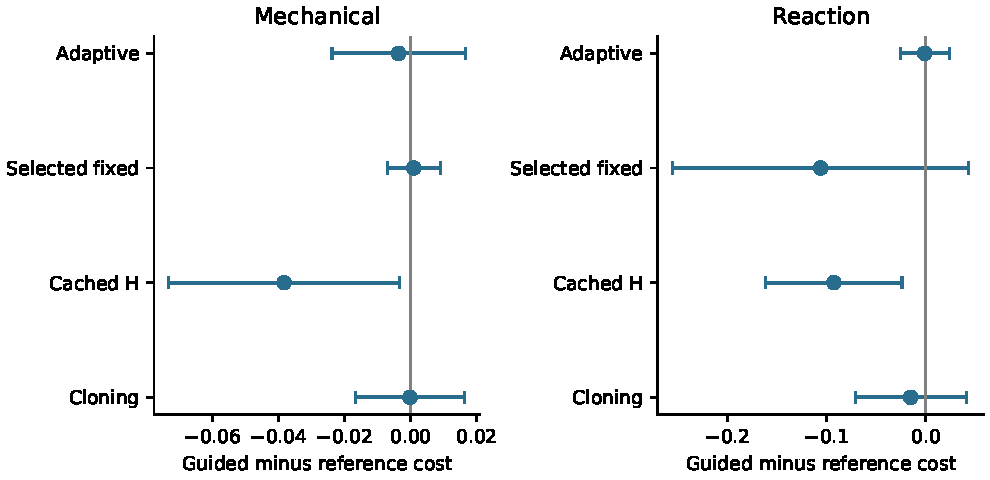
\includegraphics[width=\linewidth]{figures/impact_replication.pdf}
\caption{Audited-student minus teaching-baseline cost, with exploratory
95\% paired $t$ intervals. The adaptive baseline changes the proximal
coefficient inside the same fixed-teacher setting.}
\end{figure}

\subsection{Local diagnostics}
With fresh exact sensitivities and common $\eta=16$, the positive fitting
term exceeds the target's negative model change in both tasks. Mean
student advantage remains positive (Table~\ref{tab:decomposition}).
\begin{table}[htbp]\centering\small
\begin{tabular}{@{}lrr@{}}\toprule
Mean term & Mechanical & Reaction\\\midrule
Target-model change $-G$ & $-1.373805\times10^{-2}$ & $-2.214686\times10^{-5}$\\
Fitting contribution $R$ & $+1.415783\times10^{-2}$ & $+3.959945\times10^{-5}$\\
Nonlinear remainder $C$ & $+3.066642\times10^{-4}$ & $+1.137840\times10^{-7}$\\
Exact student advantage & $+7.264437\times10^{-4}$ & $+1.756637\times10^{-5}$\\\bottomrule
\end{tabular}
\caption{Exact accounting on 160 sampled student state/time pairs per task.
The diagnostic uses a common target coefficient and is separate from the
training-time target sequence. Terms are signed averages, not nonnegative losses.}
\label{tab:decomposition}
\end{table}
Representation, optimization, training-target differences and coverage
can all contribute; the probes do not isolate them. The fresh local
model has two false positives among 101 predicted mechanical improvements
and none among 33 reaction predictions.
\begin{figure}[htbp]\centering
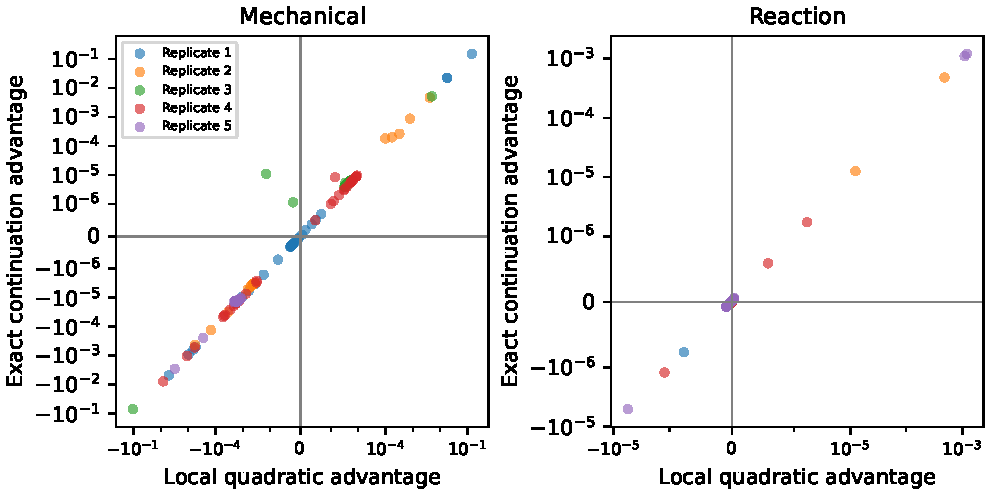
\includegraphics[width=\linewidth]{figures/current_advantage.pdf}
\caption{Local quadratic versus exact continuation advantage for the
selected audited students. Symmetric-log axes retain positive and negative
values. The upper-left quadrant contains false positive local predictions.}
\end{figure}
Among 3,840 evaluations with nonzero injected noise, the quadratic model
predicts improvement in every case and is wrong in 2,993. The empirical
margin predicts 436 improvements with no false positives, abstaining
88.65\% of the time. At reaction Gaussian magnitude 1.5 it abstains
even on four genuinely improving targets. States are reused across
conditions. Across all 4,800 evaluations there are 26 curvature-bound
violations (12 mechanical, 14 reaction), and two unperturbed mechanical
false-positive margin predictions (\ref{app:diagnostics}).
\begin{figure}[htbp]\centering
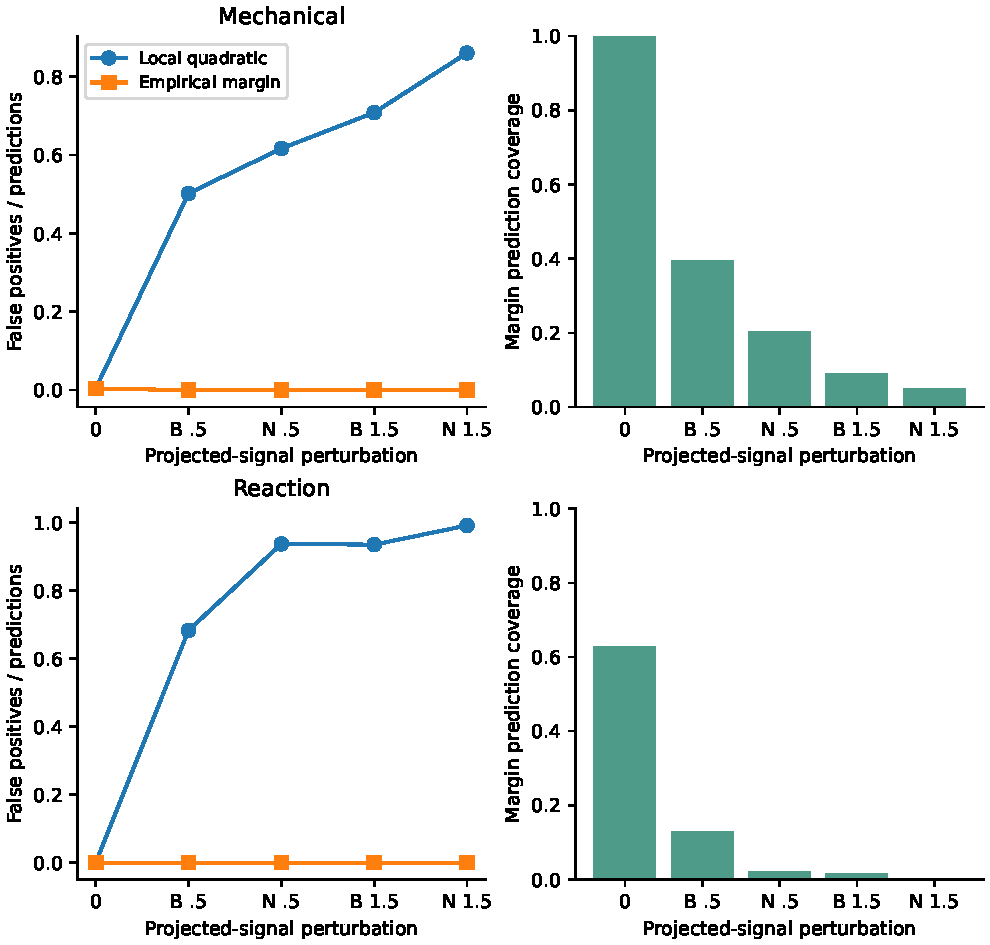
\includegraphics[width=.92\linewidth]{figures/impact_noise.pdf}
\caption{False positives and coverage under projected-sensitivity
perturbations. B denotes fixed bias and N Gaussian noise. Each task/condition
has 480 action evaluations from 160 sampled pairs across three teacher
qualities. Zero predictions in the final reaction condition denote abstention.}
\end{figure}

\subsection{Computation}
Mechanical runs request 107 fitting extensions and 50 refreshes;
reaction runs request 66 extensions, 16 refreshes and 44 regularizations.
Common preparation averages 11.54 and 14.07 seconds (38.5\% and
46.9\% of budget). Audited teaching averages 4,019 and 3,232 updates,
versus 29,770 and 21,507 for cached Hamiltonian fitting. Continuations,
the unused cached-target probe and the small refresh window impose
overhead without isolating each branch's contribution to final cost.
